\scanpage{53}
\mspage{52}

\inserted{C'est évidemment nécessaire. Pour la suffisance,} Il suffit de voir que \deleted{\unsure{cela implique}} les conditions a') b'), \deleted{\unsure{a)}} impliquent, \inserted{$f$ injectif (ce qui résulte de b') et que} pour $F',G'\in\unsure{\mathcal F'|\mathscr F'}$
\[
f(G')\leq f(F')\Longrightarrow G'\leq F'
\]

\uline{Dém} \deleted{\unsure{Par}} b'), \deleted{$\unsure{\exists\,G'}$} si $f(G')\leq f(F')$, $\exists\,\overline{G'}\leq F'$ tel que $f(\overline{G'})\deleted{\unsure{\leq}}=f(G')$. Mais alors par a on a $G'=\overline{G'}$, d'où $G'\leq F'$, \unsure{q.e.d.|p.c.d.}

\uline{Définition} On dit que l'atelier $\mathcal F$ \inserted{(satisfaisant At 1--At 8)} est \deleted{\unsure{faiblement}} \inserted{\uline{quasi}} \uline{ensembliste} (on renforcera ce ``ensembliste'' plus tard) si le comorphisme canonique
\[
\mathcal F\unsure{-|\to}\operatorname{Fig}(L)
\]
est un \uline{plongement}, ou, ce qui revient au $\unsure{=|<}$ (compte tenu de (1.53) p. 46) si on a
% slanted
\margin{Pour correctif voir \unsure{CF|GF} 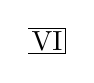
\begin{tikzpicture}[baseline=(n.base)]\node[inner sep=1pt] (n) {$\mathrm{VI}$};\draw (n.north west)--(n.north east)--(n.south east)--(n.south west);\end{tikzpicture} p. 12}
\[
\begin{aligned}
\text{\uuline{At ens 1}}\qquad &\forall\, F,G\in\mathcal F,\\
&\unsure{\operatorname{mulomb}|\operatorname{mulom}}(F)\ll\operatorname{mulomb}(G)\Longrightarrow F\ll G.
\end{aligned}
\]

\uline{Remarque} 1) On voit qu'il suffit de poser At ens 1 pour $F,G$ des multistrates $X,Y\in M$. Ce serait plus joli de poser At ens en ces termes.

2) On n'exige pas que le sous-atelier $\mathcal F\hookrightarrow\operatorname{Fig}(L)$ soit \unsure{gracieux|spacieux}. \uline{Par \unsure{exemples|exemple}} \deleted{\unsure{Considérons}} \deleted{de \unsure{l'exemple} \unsure{$B$}} \deleted{\unsure{C)}} Soit $E$ un espace topologique ou modéré, et $M$ l'ens de ses \uline{m}ultistrates \uline{simplexes} (topologiques, ou modérés), mais
